% interactcadsample.tex
% v1.03 - April 2017

\documentclass[]{interact}

\usepackage{epstopdf}% To incorporate .eps illustrations using PDFLaTeX, etc.
\usepackage{subfigure}% Support for small, `sub' figures and tables
%\usepackage[nolists,tablesfirst]{endfloat}% To `separate' figures and tables from text if required

\usepackage{natbib}% Citation support using natbib.sty
\bibpunct[, ]{(}{)}{;}{a}{}{,}% Citation support using natbib.sty
\renewcommand\bibfont{\fontsize{10}{12}\selectfont}% Bibliography support using natbib.sty

\theoremstyle{plain}% Theorem-like structures provided by amsthm.sty
\newtheorem{theorem}{Theorem}[section]
\newtheorem{lemma}[theorem]{Lemma}
\newtheorem{corollary}[theorem]{Corollary}
\newtheorem{proposition}[theorem]{Proposition}

\theoremstyle{definition}
\newtheorem{definition}[theorem]{Definition}
\newtheorem{example}[theorem]{Example}

\theoremstyle{remark}
\newtheorem{remark}{Remark}
\newtheorem{notation}{Notation}


% tightlist command for lists without linebreak
\providecommand{\tightlist}{%
  \setlength{\itemsep}{0pt}\setlength{\parskip}{0pt}}



\usepackage{lscape}
\usepackage{hyperref}
\usepackage[utf8]{inputenc}
\def\tightlist{}
\newcommand*{\Perm}[2]{{}^{#1}\!P_{#2}}%

\usepackage{booktabs}
\usepackage{longtable}
\usepackage{array}
\usepackage{multirow}
\usepackage{wrapfig}
\usepackage{float}
\usepackage{colortbl}
\usepackage{pdflscape}
\usepackage{tabu}
\usepackage{threeparttable}
\usepackage{threeparttablex}
\usepackage[normalem]{ulem}
\usepackage{makecell}
\usepackage{xcolor}

\begin{document}


\articletype{ARTICLE TEMPLATE}

\title{Why aren't significance tests commonly used for linear regression
diagnostics?}


\author{\name{Weihao Li$^{a}$, Dianne Cook$^{a}$, Emi
Tanaka$^{a}$, Susan VanderPlas$^{b}$}
\affil{$^{a}$Department of Econometrics and Business Statistics, Monash
University, Clayton, VIC, Australia; $^{b}$Department of Statistics,
University of Nebraska, Lincoln, Nebraska, USA}
}

\thanks{CONTACT Weihao
Li. Email: \href{mailto:weihao.li@monash.edu}{\nolinkurl{weihao.li@monash.edu}}, Dianne
Cook. Email: \href{mailto:dicook@monash.edu}{\nolinkurl{dicook@monash.edu}}, Emi
Tanaka. Email: \href{mailto:emi.tanaka@monash.edu}{\nolinkurl{emi.tanaka@monash.edu}}, Susan
VanderPlas. Email: \href{mailto:susan.vanderplas@unl.edu}{\nolinkurl{susan.vanderplas@unl.edu}}}

\maketitle

\begin{abstract}
Abstract to fill.
\end{abstract}

\begin{keywords}
data visualization; visual inference; hypothesis testing; residual
plots;
\end{keywords}

\hypertarget{introduction}{%
\section{Introduction}\label{introduction}}

\begin{quote}
\emph{``Since all models are wrong the scientist must be alert to what
is importantly wrong.''} \citep{box1976science}
\end{quote}

Diagnosing a model is the key to determining whether there is anything
importantly wrong. For linear regression analysis, we typically
interrogate the residuals for model diagnostics. Residuals summarise
what is not captured by the model, and thus provide the capacity to
identify what might be wrong.

We can assess residuals in multiple ways. Residuals might be plotted, as
a histogram or quantile-quantile plot to examine the distribution. Using
the classical normal linear regression model as an example, if the
distribution is symmetric and unimodal, it is well-behaved. But if the
distribution is skewed, bimodal, multimodal, or contains outliers, there
is cause for concern. The distribution could also be inspected by
conducting a goodness of fit test, such as the Shapiro-Wilk Normality
test \citep{shapiro1965analysis}.

Plotting the residuals against predicted values and each of the
explanatory variables on a scatter plot is a recommend way to scrutinize
their relationships. If there is any visually discoverable patterns, the
model is potentially misspecified. However, correctly judging a residual
plot where no pattern exists is a painstakingly difficult task for
humans.

It is especially common, particularly among new data analytics students
to report patterns when an experienced data analyst might quickly
conclude that there are none. {[}ET: I don't know if the former
statement is true? \textgreater\textgreater{} PL: change to students{]}
Generally, one looks for noticeable departures from the model like
non-linear dependency or heteroskedasticity. It is also possible to
conduct hypothesis tests for non-linear dependence
\citep{ramsey_tests_1969}, and use a Breusch-Pagan test
\citep{breusch_simple_1979} for heteroskedasticity.

Abundance of literature describe appropriate diagnostic methods for
linear regression: \citet{draper1998applied},
\citet{montgomery1982introduction}, \citet{belsley_regression_1980},
\citet{cook_applied_1999} and \citet{cook1982residuals}. The diligent
reader of these sage writings will also notice sentences that express
sentiments like \emph{based on their experience, statistical tests are
not widely used in regression diagnostics. The same or even larger
amount of information can be provided by diagnostic plots than the
corresponding tests in most empirical studies.} A common guidance by
experts is that optimal method for diagnosing model fits is by plotting
the data.

The persistence of this advice to check the plots is curious, and
investigating why this might be common advice is the subject of this
paper. The paper is structured as follows. The next background section
describes the types of departures that one expects to detect, and
describes a formal statistical process for reading residual plots,
called visual inference {[}ET: CITATION HERE? \textgreater\textgreater{}
PL: arguments removed{]}. Section \ref{experimental-design} describes
the experiment design to compare the decision made by formal hypothesis
testing, and how humans would read diagnostic plots. The results are
reported in Section \ref{results}. We finish with a discussion on future
work, in particular how the responsibility for residual plot reading
might be passed on to computer vision.

\hypertarget{background}{%
\section{Background}\label{background}}

\hypertarget{departures-from-good-residual-plots}{%
\subsection{Departures from good residual
plots}\label{departures-from-good-residual-plots}}

\begin{figure}

{\centering 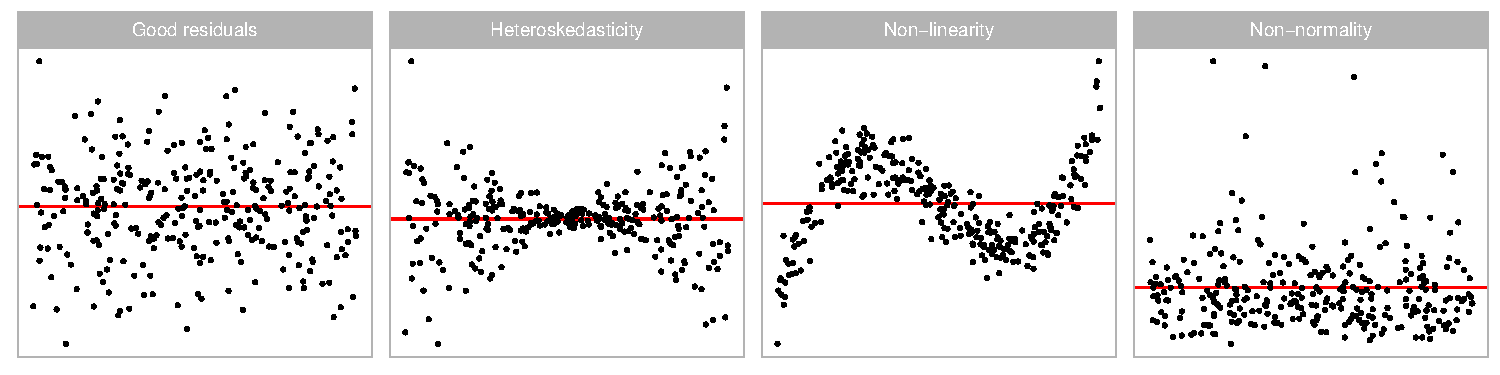
\includegraphics[width=1\linewidth]{paper_comparison_files/figure-latex/residual-plot-common-departures-1} 

}

\caption{Example fitted vs residual plots: (A) classically good looking residuals, (B) non-linear pattern indicates that the model has not captured a non-linear association, (C) heteroskedasticity indicating that variance around the fitted model is not uniform, and (D) non-normality where the residual distribution is not symmetric around 0. The latter pattern might best be assessed using a univariate plot of the residuals, but patterns B and C need to be assessed using a residual vs fitted plot.}\label{fig:residual-plot-common-departures}
\end{figure}

Graphical summaries in which residuals are plotted against fitted values
or other functions of the regressors that are approximately orthogonal
to residuals are referred to as standard residual plots in
\citet{cook1982residuals}. As shown in Figure
\ref{fig:residual-plot-common-departures}, the top-left panel is a good
residual plot with residuals evenly distributed at both sides of the
horizontal zero line showing no noticeable patterns.

There are various types of departures from a good residual plot.
Non-linearity, heterskedasticity and non-normality are perhaps the three
mostly checked departures.

Non-linearity is a type of model misspecification caused by failing to
include higher order terms of the regressors in the regression equation.
Any non-linear functional form of residuals on fitted values presented
in the residual plot could be considered as an indicative of
non-linearity. An example residual plot containing visual pattern of
non-linearity is given at plot B of Figure
\ref{fig:residual-plot-common-departures}. One can clearly observe the
``S-shape'' from the residual plot as the cubic term is not captured by
the misspecified model.

Heteroskedasticity refers to the presence of nonconstant error variance
in a regression model. It is mostly due to the strict but false
assumptions on the variance-covariance matrix of the error term. The
usual pattern of heteroskedasticity on a residual plot is the
inconsistent spread of the residuals across the horizontal axis.
Visually, it sometimes results in the so-called ``butterfly'' shape as
shown in the plot C of Figure \ref{fig:residual-plot-common-departures},
or the ``left-triangle'' and ``right-triangle'' shape where the smallest
variance occurs at one side of the horizontal axis.

Compared to non-linearity and heteroskedasticity, non-normality is
usually harder to detect from a residual plot since scatter plot do not
readily reveal the marginal distribution. A favourable graphical summary
for this task is the quantile-quantile plot. However, for a consistent
comparison, residual plot will be the focus of this paper. Besides, it
is important to note that not all regression models assume normality for
the error term, but a certain amount do including the classical normal
linear regression model. In the case that the normality assumption is
violated, it is expected to observe data points do not center around the
horizontal axis and there is an uneven distribution of the number points
at both below and above the horizontal axis. For example, given a skewed
error distribution, fewer data points and more outliers are on one side
of the horizontal axis as shown in plot D of Figure
\ref{fig:residual-plot-common-departures}.

\hypertarget{conventionally-testing-for-departures}{%
\subsection{Conventionally testing for
departures}\label{conventionally-testing-for-departures}}

Other than checking diagnostic plots, analysts may perform formal
hypothesis testing for detecting model defects. Depending on the
alternative hypothesis that is focused on, a variety of tests can be
applied. For example, the presence of heteroskedasticity can usually be
tested by applying the White test
\citep{white_heteroskedasticity-consistent_1980} or the Breusch-Pagan
test \citep{breusch_simple_1979}, which are both derived from the
Lagrange multiplier test \citep{silvey1959lagrangian} principle that
relies on the asymptotic properties of the null distribution. For
testing non-linearity, one may apply the F-test as a model structural
test to examine the significance of specific polynomial and non-linear
forms of the regressors, or the significance of proxy variables as in
the Ramsey Regression Equation Specification Error Test (RESET)
\citep{ramsey_tests_1969}. And for testing normality, the Shapiro--Wilk
test \citep{shapiro1965analysis} is perhaps the most widely used test
included by many of the statistical softwares. Another choice will be
the Jarque--Bera test \citep{jarque1980efficient} which directly checks
if the sample skewness and kurtosis match a normal distribution.

Example residual plots given in Figure
\ref{fig:residual-plot-common-departures} are examined by the
corresponding RESET test, Breusch-Pagan test and Shapiro--Wilk test as
shown in Table \ref{tab:example-residual-plot-table}. In the example,
both the Breusch-Pagan test and the Shapiro--Wilk test rejects the null
hypothesis \(H_0\) for departures that they do not intend to examine. As
discussed in \citet{cook1982residuals}, most residual-based tests for a
particular type of departure from model assumptions are sensitive to
other types of departures. It is likely \(H_0\) is correctly rejected
but for the wrong reason, which is known as the ``Type III error''.
Additionally, outliers will often incorrectly trigger the rejection of
\(H_0\) despite when majority of the residuals are well-behaved
\citep{cook_applied_1999}. Furthermore, with a sufficiently large sample
size, residual-based tests may reject \(H_0\) due to a slight departure
that is of little practical significance. These can be largely avoided
in diagnostic plots as experienced analysts can evaluate the
acceptability of assumptions flexibly, even in the presence of outliers
and slight departures.

\begin{table}

\caption{\label{tab:example-residual-plot-table}Statistical significance testing for departures from good residuals for plots in Figure \ref{fig:residual-plot-common-departures}. Shown are the $p$-values calculated for the conventional RESET, the Breusch-Pagan and the Shapiro–Wilk tests. The good residual plot (A) is judged a good residual plot, as expected, by all tests. The non-linearity (B) is detected by all tests, as might be expected given the extreme structure.}
\centering
\begin{tabular}[t]{llrrr}
\toprule
Plot & Departures & RESET & Breusch-Pagan & Shapiro–Wilk\\
\midrule
A & None & 0.779 & 0.133 & 0.728\\
B & Non-linearity & \em{0.000} & \em{0.000} & \em{0.039}\\
C & Heteroskedasticity & 0.658 & \em{0.000} & \em{0.000}\\
D & Non-normality & 0.863 & 0.736 & \em{0.000}\\
\bottomrule
\end{tabular}
\end{table}

\hypertarget{visual-testing-for-departures}{%
\subsection{Visual testing for
departures}\label{visual-testing-for-departures}}

\hypertarget{lineup-protocol}{%
\subsubsection{Lineup protocol}\label{lineup-protocol}}

One may argue that reading diagnostic plots is to some extent subjective
and indecisive compared to those rigorous statistical procedures as it
relies on graphical perception - human's ability to interpret and decode
the information embedded in the graph \citep{cleveland_graphical_1984}.
It is particularly true that visual discovery suffers from its unsecured
and unconfirmed nature where the degree of the presence of the visual
features typically can not be measured quantitatively and objectively,
which may lead to over or under-interpretations of the data. One such
example is finding an over-interpretation of the separation between gene
groups in a two-dimensional projection from a linear discriminant
analysis when in fact there are no differences in the expression levels
between the gene groups and separation is not an uncommon occurrence
\citep{roy_chowdhury_using_2015}.

Visual inference was first introduced in a 1999 Joint Statistical
Meetings (JSM) talk with the title ``Inference for Data Visualization''
by \citet{buja_inference_1999} as an idea to address the issue of valid
inference for visual discoveries of data plots
\citep{gelman_exploratory_2004}. Later, \citet{buja_statistical_2009}
proposed the lineup protocol as a visual test inspired by the ``police
lineup'' or ``identity parade'' which is the act of asking the
eyewitness to identify criminal suspect from a group of irrelevant
people. The protocol consists of \(m\) randomly placed plots, where one
plot is the actual data plot, and the remaining \(m - 1\) plots have the
identical graphical production as the data plot except the data has been
replaced with data consistent with \(H_0\). Then, an observer who have
not seen the actual data plot will be asked to point out the most
different plot from the lineup. Under \(H_0\), it is expected that the
actual data plot would have no distinguishable difference with the null
plots, and the probability of the observer correctly picks the actual
data plot is \(1/m\). If we reject \(H_0\) as the observer correctly
picks the actual data plot, then the Type I error of this test is
\(1/m\).

\begin{figure}

{\centering 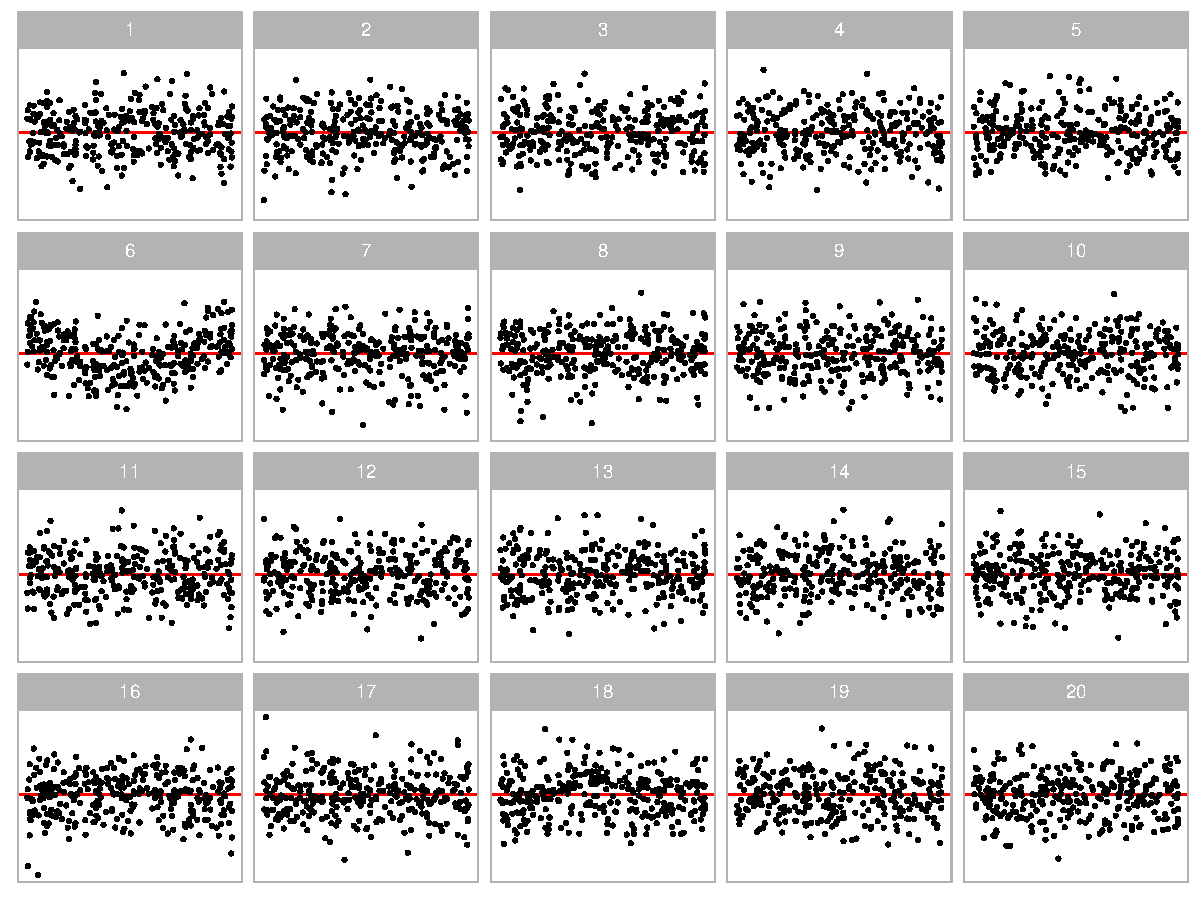
\includegraphics[width=1\linewidth]{paper_comparison_files/figure-latex/first-example-lineup-1} 

}

\caption{Visual testing is conducted using a lineup, as in the example here. The residual plot computed from the observed data (plot 7, exhibiting non-linearity) is embedded among 19 null plots, where the residuals were simulated from a standard error model. Computing the $p$-value requires that the lineup be examined by a number of human judges, each asked to select the most different plot. A small $p$-value would result from a substantial number selecting plot 7.}\label{fig:first-example-lineup}
\end{figure}

Figure \ref{fig:first-example-lineup} is an example of a lineup
protocol. If the actual data plot at position 7 is identifiable, then it
is evidence for the rejection of \(H_0\) that the regression model is
correctly specified. In fact, the actual residual plot is obtained from
a misspecified regression model with non-linearity issue.

The effectiveness of lineup protocol is validated by
\citet{majumder_validation_2013} under relatively simple classical
normal linear regression model settings with one or two regressors.
Their results suggest visual test is capable of testing the significance
of a single regressor with a similar power as a t-test, though they
expressed that in general it is unnecessary to use visual inference if
there exists a conventional test and they didn't expect the visual test
to perform equally well as the conventional test. In their third
experiment, where there does not exist a proper conventional test,
visual test outperforms the conventional test for a large margin. This
is encouraging as it promotes the use of visual inference in border
field of data science where there are no existing statistical testing
procedures. Visual inference have also been integrated into diagnostic
of hierarchical linear models by \citet{loy2013diagnostic},
\citet{loy2014hlmdiag} and \citet{loy2015you}. They use lineup protocols
to judge the assumption of linearity, normality and constant error
variance for both the level-1 and level-2 residuals.

\hypertarget{sampling-from-the-null-distribution}{%
\subsubsection{Sampling from the null
distribution}\label{sampling-from-the-null-distribution}}

Data used in the \(m - 1\) null plots need to be simulated. In the
context of regression diagnostics, sampling data from \(H_0\) is
equivalent to sampling data from the assumed model. As
\citet{buja_statistical_2009} suggest, \(H_0\) is usually composited by
a collection of distributions controlled by nuisance parameters. Since
regression models can have various forms, there is no general solution
to this problem, but it sometimes can be reduced to so called
``reference distribution'' by applying one of the three methods: (i)
sampling from a conditional distribution given a minimal sufficient
statistic under \(H_0\), (ii) parametric bootstrap sampling with
nuisance parameters estimated under \(H_0\), and (iii) Bayesian
posterior predictive sampling. The conditional distribution given a
minimal sufficient statistic is the best justified reference
distribution among the three \citep{buja_statistical_2009}. Essentially,
null residuals can be simulated by regressing \(N\) i.i.d standard
normal random draws on the regressors, then rescaling it by the ratio of
residual sum of square in two regressions.

\hypertarget{calculating-p-values}{%
\subsubsection{\texorpdfstring{Calculating
\(p\)-values}{Calculating p-values}}\label{calculating-p-values}}

Further, a visual test can involve \(K\) independent observers. Let
\(X_i = \{0,1\}\) be a binomial random variable denoting whether subject
\(i\) correctly detecting the actual data plot, and
\(X = \sum_{i=1}^{K}X_i\) be the number of observers correctly picking
the actual data plot. Then, by imposing a relatively strong assumption
on the visual test that all \(K\) evaluations are fully independent,
under \(H_0\), \(X \sim \mathrm{Binom}_{K,1/m}\). Therefore, the
\(p\)-value of a lineup of size \(m\) evaluated by \(K\) observer is
given as \(P(X \geq x) = 1 - F(x) + f(x)\), where \(F(.)\) is the
cumulative distribution function, \(f(.)\) is the probability mass
function and \(x\) is the realization of number of observers correctly
picking the actual data plot \citep{majumder_validation_2013}.

As point out by \citet{vanderplas2021statistical}, this basic binomial
model doesn't take into account the possible dependencies in the visual
test due to repeated evaluations of the same lineup. And it is
inapplicable to visual test where subjects are asked to select one or
more ``most different'' plots from the lineup.
\citet{vanderplas2021statistical} summarizes three common scenarios in
visual inference: (1) \(K\) different lineups are shown to \(K\)
subjects, (2) \(K\) lineups with different null plots but the same
actual data plot are shown to \(K\) subjects, and (3) the same lineup is
shown to \(K\) subjects. Out of these three scenarios, Scenario 3 is the
most common in previous studies as it puts the least constraints on the
experiment design. For Scenario 3, \citet{vanderplas2021statistical}
model the probability of a plot \(i\) being selected from a lineup as
\(\theta_i\), where \(\theta_i \sim Dirichlet(\alpha)\) for
\(i=1,...,m\) and \(\alpha > 0\). And defined \(c_i\) to be the number
of times plot \(i\) being selected in \(K\) evaluations. In case subject
\(j\) makes multiple selections, \(1/s_j\) will be added to \(c_i\)
instead of one, where \(s_j\) is the number of plots subject \(j\)
selected for \(j=1,...K\). This ensured \(\sum_{i}c_i=K\). Since we are
only interested in the selections of the actual data plot \(i\), the
marginal model can be simplified to a beta-binomial model and thus the
visual p-value is given as

\begin{equation} \label{eq:pvalue-beta-binomial}
P(C \geq c_i) = \sum_{x=c_i}^{K}{K \choose x}\frac{B(x + \alpha, K - x + (m - 1)\alpha)}{B(\alpha, (m-1)\alpha)},\quad \text{for} \quad c_i \in \mathbb{Z}_0^+
\end{equation}

\noindent where \(B(.)\) is the beta function defined as

\begin{equation} \label{eq:betafunction}
B(a, b) = \int_{0}^{1}t^{\alpha - 1}(1-t)^{b-1}dt,\quad \text{where}\quad a,b>0. 
\end{equation}

Note that Equation \ref{eq:pvalue-beta-binomial} only works with
non-negative integer \(c_i\). For non-negative real number \(c_i\),
linear approximation will be applied to calculate the p-value

\begin{equation} \label{eq:pvalue-beta-binomial-approx}
P(C \geq c_i) = P(C \geq \lceil c_i \rceil) + (\lceil c_i \rceil - c_i) P(C = \lfloor c_i \rfloor), \quad \text{for}\quad c_i \in \mathbb{R}_0^+,
\end{equation}

where \(P(C \geq \lceil c_i \rceil)\) is calculated using Equation
\ref{eq:pvalue-beta-binomial} and \(P(C = \lfloor c_i \rfloor)\) is
calculated by

\begin{equation}
P(C = c_i) = {K \choose c_i}\frac{B(c_i + \alpha, K - c_i + (m - 1)\alpha)}{B(\alpha, (m-1)\alpha)},\quad \text{for} \quad c_i \in \mathbb{Z}_0^+.
\end{equation}

Besides, the parameter \(\alpha\) used in Equation
\ref{eq:pvalue-beta-binomial} is usually unknown and hence needs to be
estimated from the survey data. For low values of \(\alpha\), only a few
plots are attractive to the observers and tend to be selected. For
higher values of \(\alpha\), the distribution of the probability of each
plot being selected is more even. \citet{vanderplas2021statistical}
define that a plot is \(c\)-interesting if \(c\) or more participants
select the plot as the most different. Given the definition, The
expected number of plots selected at least \(c\) times, \(E[Z_c]\), is
calculated as

\begin{equation} \label{eq:c-interesting-expectation}
E[Z_c(\alpha)] = \frac{m}{B(\alpha, (m-1)\alpha)}\sum_{\lceil c \rceil}^{K}{K \choose x} B(x + \alpha, K - x + (m-1)\alpha).\end{equation}

\citet{vanderplas2021statistical} suggest that \(\alpha\) can be
estimated using MLE with Equation \ref{eq:c-interesting-expectation}.
But for precise estimate of \(\alpha\), additional responses to
Rorschach lineups, which is a type of lineup consists of only null
plots, are required.

\hypertarget{power-calculation}{%
\subsubsection{Power calculation}\label{power-calculation}}

As discussed in \citet{majumder_validation_2013}, individual's skill
will affect the number of observers who identify the actual data plot
from the lineup. Thus, the power of a visual test depends on the
subject-specific abilities. Previously, it was addressed by modelling
the probability of a subject \(i\) correctly picking the actual data
plot from a lineup \(l\) using a mixed-effect logistic regression with
the subject being treated as a random effect
\citep{majumder_validation_2013}. However, having this probability is
insufficient to determine the power of a visual test allowed for
multiple selections as it doesn't provide information about the number
of selections made by the subject for p-value calculation.

Instead, we directly estimated the probability of a lineup being
rejected using a logistic regression with the natural logarithm of the
effect size as the only regressor formulated as

\begin{equation} \label{eq:logistic-regression-1-1}
Pr(\text{reject}~H_0|H_1,E) = \Lambda(\beta_0 + \beta_1 log_e(\boldsymbol{E})),
\end{equation}

\noindent where \(\Lambda(.)\) is the standard logistic function given
as \(\Lambda(z) = exp(z)/(1+exp(z))\).

Effect \(E\) is derived from the Kullback-Leibler divergence (see
{[}appendix ref here{]}) formulated as

\begin{equation} \label{eq:effect-size-ex1}
E = \frac{1}{2\sigma^2}\boldsymbol{X}_b'\boldsymbol{R}_a'(diag(\boldsymbol{R}_a))^{-1}\boldsymbol{R}_a\boldsymbol{X}_b,
\end{equation}

\noindent where \(diag(.)\) is the diagonal matrix constructed from the
diagonal elements of \(\boldsymbol{R}_a\).

To study various factors contributing to the power of the visual test,
the same logistic regression model is fit on different subsets of the
collated data grouped by levels of factors. This includes
{[}expansion{]}.

\hypertarget{experimental-design}{%
\section{Experimental design}\label{experimental-design}}

(This section discusses the experimental design including the motivation
of the experiment, an overview of the experiment, the simulation setting
of the depatures from good residual plots, parameter choices, allocation
of the lineups and other technical details.)

Three experiments were conducted to investigate the difference between
conventional hypothesis testing and visual inference in the application
of linear regression diagnostics. The experiment I has ideal scenario
for conventional testing, where the visual test is not expected to
outperform the conventional test. Meanwhile, the experiment II is a
scenario where the conventional test is an approximate test, in which
the visual test may have a chance to match the performance of the
conventional test. The experiment III is designed for collecting human
responses to lineup with only good residual plots such that the
parameter \(\alpha\) in Equation \ref{eq:pvalue-beta-binomial} can be
estimated. Overall, we planned to collect 7974 evaluations on 1152
uniqued lineups performed by 443 subjects throughout three experiment.

\hypertarget{simulating-departures}{%
\subsection{Simulating departures}\label{simulating-departures}}

Two types of departures, namely non-linearity and heteroskedasticity,
were considered with the corresponding data generating process being
designed for experiment I and II.

\hypertarget{non-linearity}{%
\subsubsection{Non-linearity}\label{non-linearity}}

\begin{figure}

{\centering 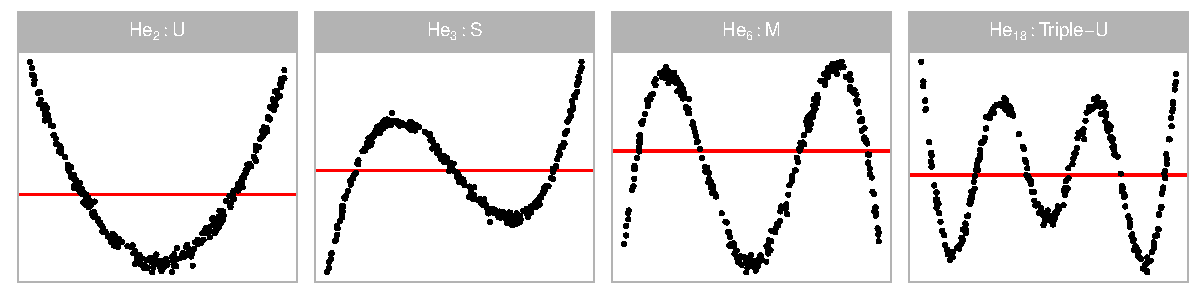
\includegraphics[width=1\linewidth]{paper_comparison_files/figure-latex/different-shape-of-herimite-1} 

}

\caption{Polynomial forms generated for the residual plots used in experiment I. The four shapes are generated by varying the order of polynomial given by $j$ in $He_j(.)$.}\label{fig:different-shape-of-herimite}
\end{figure}

Experiment I is designed to study the ability of human subjects to
detect the effect of a non-linear term \(\boldsymbol{z}\) constructed
using Hermite polynomials {[}Hermite ref here{]} on random vector
\(\boldsymbol{x}\) formulated as

\begin{align} \label{eq:nonlinearity-model}
\boldsymbol{y} = 1 + \boldsymbol{x} + \boldsymbol{z} + \boldsymbol{\varepsilon},\\
\boldsymbol{x} = g(\boldsymbol{x}_{raw}, 1), \\
\boldsymbol{z} = g(\boldsymbol{z}_{raw}, 1), \\
\boldsymbol{z}_{raw} = He_j(g(\boldsymbol{z}, 2)),
\end{align}

\noindent where \(\boldsymbol{y}\), \(\boldsymbol{x}\),
\(\boldsymbol{\varepsilon}\), \(\boldsymbol{x}_{raw}\),
\(\boldsymbol{z}_{raw}\) are vectors of size \(n\), \(He_{j}(.)\) is the
\(j\)th-order probabilist's Hermite polynomials,
\(\varepsilon \sim N(\boldsymbol{0}, \sigma^2\boldsymbol{I}_n)\), and
\(g(\boldsymbol{x}, k)\) is a scaling function to enforce the support of
the random vector to be \(\{-k, k\}\) defined as

\begin{equation} \label{eq:scaling-function}
g(\boldsymbol{x}, k) = (\boldsymbol{x} - min(\boldsymbol{x}))/max(\boldsymbol{x} - min(\boldsymbol{x}))2k - k, \quad \text{for} \quad k > 0. 
\end{equation}

The null regression model used to fit the realizations generated by the
above model is formulated as

\begin{equation} \label{eq:null-model}
\boldsymbol{y} = \beta_0 + \beta_1 \boldsymbol{x} + \boldsymbol{u},
\end{equation}

\noindent where
\(\boldsymbol{u} \sim N(\boldsymbol{0}, \sigma^2\boldsymbol{I}_n)\).

Since \(z = O(x^j)\), for \(j > 1\), \(z\) is a higher order term leaves
out by the null regression, which will result in model misspecification.
Visual patterns of non-linearity were simulated using four different
order of probabilist's Hermite polynomials (\(j = 2, 3, 6, 18\)) and
four different distribution of \(X_{raw}\): (1) \(U(-1, 1)\), (2)
\(N(0, 0.3^2)\), (3) \(lognormal(0, 0.6^2)/3\) and (4) \(u\{1, 5\}\). A
summary of the factors is given in Table \ref{tab:model-factor-table}.

\begin{table}

\caption{\label{tab:model-factor-table}Description of all factors involved in the nonlinear and heteroskedasticity studies.}
\centering
\resizebox{\linewidth}{!}{
\begin{tabular}[t]{rcrrrr}
\toprule
\multicolumn{1}{c}{Poly Order ($j$)} & \multicolumn{1}{c}{\makecell[c]{Distribution of $X_{raw}$\\}} & \multicolumn{1}{c}{SD ($\sigma$)} & \multicolumn{1}{c}{Poly Shape ($a$)} & \multicolumn{1}{c}{Heteroskedasticity ($b$)} & \multicolumn{1}{c}{Size ($n$)} \\
\cmidrule(l{3pt}r{3pt}){1-1} \cmidrule(l{3pt}r{3pt}){2-2} \cmidrule(l{3pt}r{3pt}){3-3} \cmidrule(l{3pt}r{3pt}){4-4} \cmidrule(l{3pt}r{3pt}){5-5} \cmidrule(l{3pt}r{3pt}){6-6}
2 & $U(-1, 1)$ & 0.25 & -1 & 0.25 & 50\\
3 & $N(0, 0.3^2)$ & 1.00 & 0 & 1.00 & 100\\
6 & $lognormal(0, 0.6^2)/3$ & 2.00 & 1 & 4.00 & 300\\
18 & $U\{1, 5\}$ & 4.00 &  & 16.00 & \\
 & NA &  &  & 64.00 & \\
\bottomrule
\end{tabular}}
\end{table}

The values of \(j\) was chosen so that distinct shapes of non-linearity
were included in the residual plot. A greater value of \(j\) will result
in a curve with more turning points. As shown in Figure
\ref{fig:different-shape-of-herimite}, it includes ``U'' shape, ``S''
shape, ``M'' shape and ``Triple-U'' shape. It is expected that the ``U''
shape will be the easiest one to detect because complex shape tends to
be concealed by cluster of data points.

Four different distribution were used to generate \(X_{raw}\) as shown
in Figure \ref{fig:different-dist}. The uniform and the normal
distribution are symmetric and commonly assumed in statistical models.
The adjusted log-normal distribution provides skewed density, while the
discrete uniform distribution provides discreteness in residual plot,
which could enrich the pool of visual patterns.

\begin{figure}

{\centering 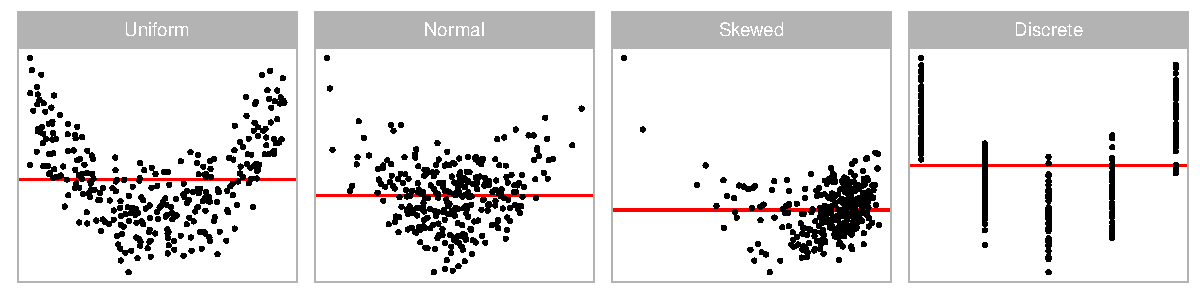
\includegraphics[width=1\linewidth]{paper_comparison_files/figure-latex/different-dist-1} 

}

\caption{Variations in fitted values, that might affect perception of residual plots. Four different distribution of $x_{raw}$ are used in the experiment to provide various visual patterns.}\label{fig:different-dist}
\end{figure}

Figure \ref{fig:example-poly-lineup} shows one of the lineups used in
experiment I. This lineup was produced under \(j = 6\) and
\(X_{raw} \sim N(0.0.3^2)\). The actual data plot location was four. All
five subjects correctly identified the actual data plot for this lineup.

\begin{figure}

{\centering 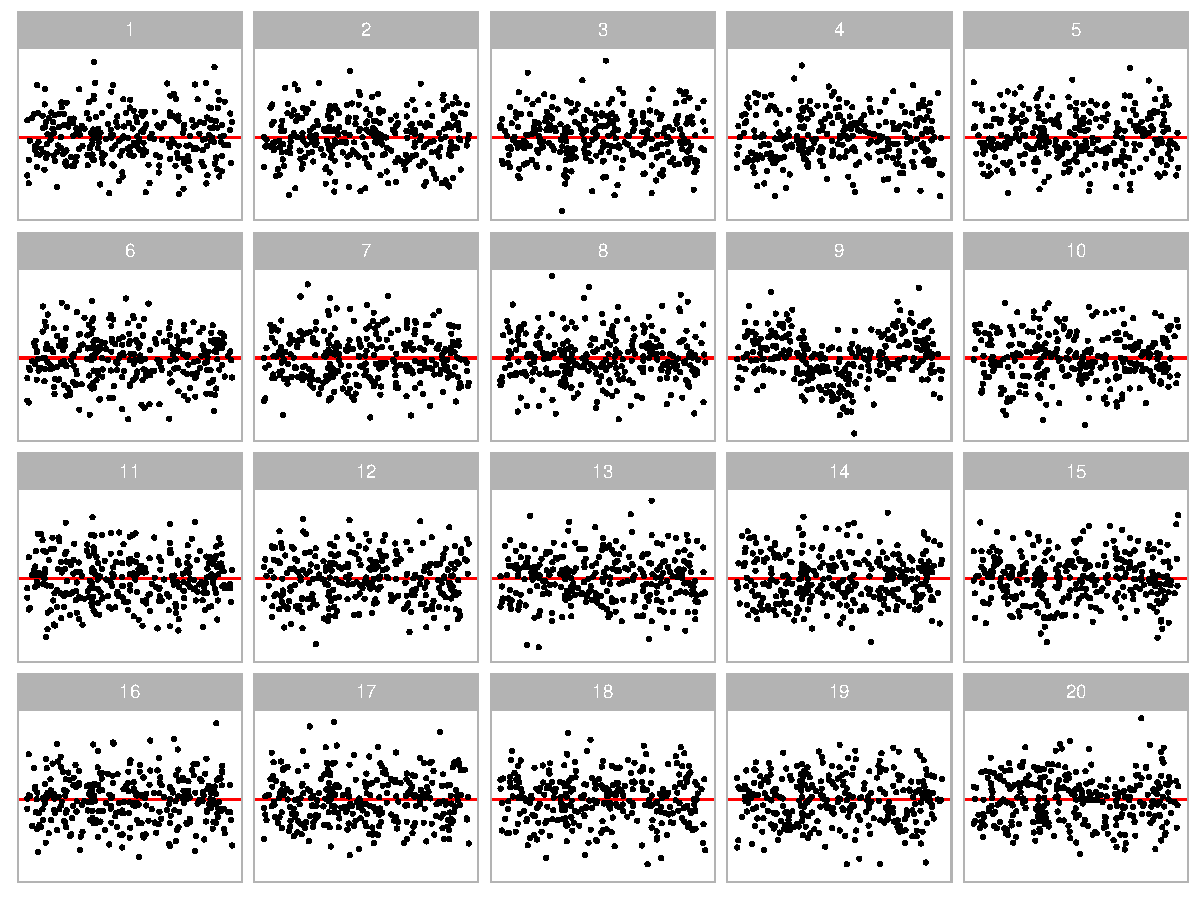
\includegraphics[width=1\linewidth]{paper_comparison_files/figure-latex/example-poly-lineup-1} 

}

\caption{Lineup poly-24 in experiment I. Can you spot the most different plot? \label{fig:example-poly-lineup}}\label{fig:example-poly-lineup}
\end{figure}

\hypertarget{heteroskedasticity}{%
\subsubsection{Heteroskedasticity}\label{heteroskedasticity}}

Experiment II is designed to study the ability of human subjects to
detect the appearance of a heteroskedasticity pattern under a simple
linear regression model setting:

\begin{align} \label{eq:heter-model}
\boldsymbol{y} = 1 + \boldsymbol{x} + \boldsymbol{\varepsilon},\\
\boldsymbol{x} = g(\boldsymbol{x}_{raw}, 1)\\
\boldsymbol{\varepsilon} \sim N(\boldsymbol{0}, 1 + 2 - |a| b (\boldsymbol{x} - a)^2 \boldsymbol{I}), \\
\end{align}

\noindent where \(\boldsymbol{y}\), \(\boldsymbol{x}\),
\(\boldsymbol{\varepsilon}\) are vectors of size \(n\) and \(g(.)\) is
the scaling function defined in \ref{eq:scaling-function}.

The null regression model used to fit the realizations generated by the
above model is formulated exactly the same as Equation
\ref{eq:null-model}.

For \(b \neq 0\), the variance-covariance matrix of the error term
\(\boldsymbol{\varepsilon}\) is correlated with the regressor \(x\),
which will lead to the presence of heteroskedasticity. Visual patterns
were simulated using three different shapes (\(a\) = -1, 0, 1) and the
same four different distribution of \(X_{raw}\) used in experiment I. A
summary of the factors is given in Table \ref{tab:model-factor-table}.

The values of \(a\) was chosen so that different shapes of
heteroskedasticity were included in the residual plot. These include
left-triangle shape, butterfly shape and right-triangle shape as
displayed in Figure \ref{fig:different-shape-of-heter}.

\begin{figure}

{\centering 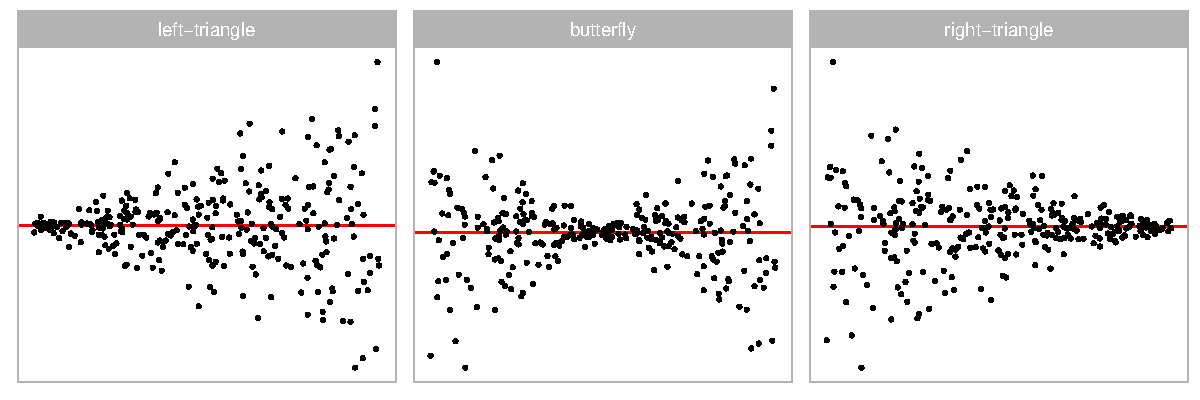
\includegraphics[width=1\linewidth]{paper_comparison_files/figure-latex/different-shape-of-heter-1} 

}

\caption{Heteroskedasticity forms used in experiment II. Three different shapes (a = -1, 0, 1) are used in the experiment to create left-triangle, butterfly and right-triangle shapes.}\label{fig:different-shape-of-heter}
\end{figure}

\begin{figure}

{\centering 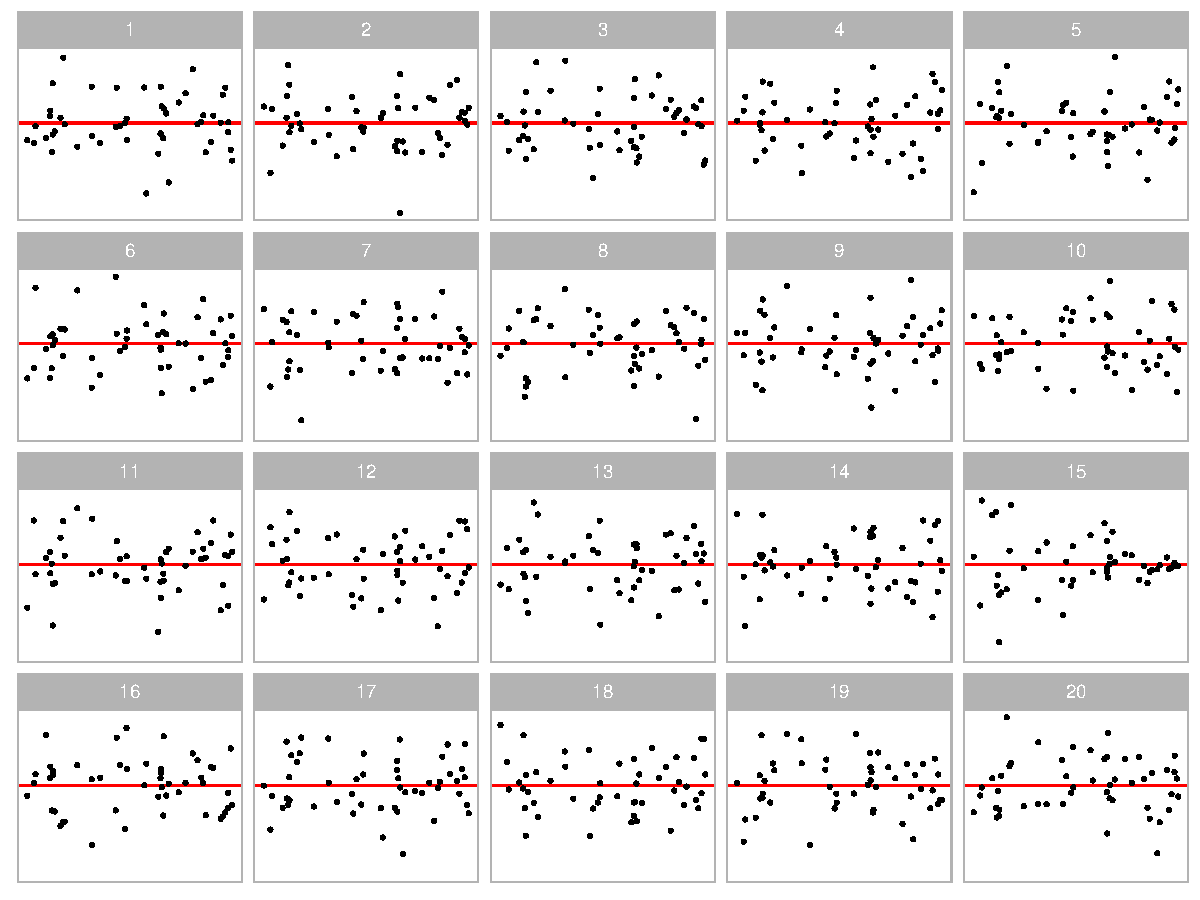
\includegraphics[width=1\linewidth]{paper_comparison_files/figure-latex/example-heter-lineup-1} 

}

\caption{Lineup heter-169 in experiment II. Can you spot the most different plot? \label{fig:example-heter-lineup}}\label{fig:example-heter-lineup}
\end{figure}

An example lineup of this model is shown in Figure
\ref{fig:example-heter-lineup} with \(a = -1\) and
\(X_{raw} \sim U(-1, 1)\). The actual data plot location was 15. 8 out
of 11 subjects correctly identified the actual data plot for this
lineup.

\hypertarget{experimental-setup}{%
\subsection{Experimental setup}\label{experimental-setup}}

\hypertarget{controlling-the-strength-of-the-signal}{%
\subsubsection{Controlling the strength of the
signal}\label{controlling-the-strength-of-the-signal}}

As summarised in Table \ref{tab:model-factor-table}, three additional
parameters \(n\), \(\sigma\) and \(b\) were used to control the strength
of the signal so that different difficulty levels of lineups were
generated, and therefore, the estimated power curve would be smooth and
continuous. Parameter \(\sigma \in \{0.5, 1, 2, 4\}\) and
\(b \in \{0.25, 1, 4, 16, 64\}\) were used in experiment I and II
respectively. Figure \ref{fig:different-sigma} and \ref{fig:different-b}
demonstrate the impact of these two parameters. A large value of
\(\sigma\) will increase the variation of the error of the non-linear
model and decrease the visibility of the visual pattern. The parameter
\(b\) controls the ratio of the standard deviation of the
heteroskedasticity across the domain of the regressor. Given
\(x \neq a\), a larger value of \(b\) will lead to a larger ratio of the
variance at \(x\) to the variance at \(x - a = 0\), making the visual
pattern more obvious.

Three different sample sizes were used (n = 50, 100, 300) in all three
experiments. It can be observed from Figure \ref{fig:different-n} that
with fewer data points drawn in a residual plot, the visual pattern is
more difficult to be detected.

\begin{figure}

{\centering 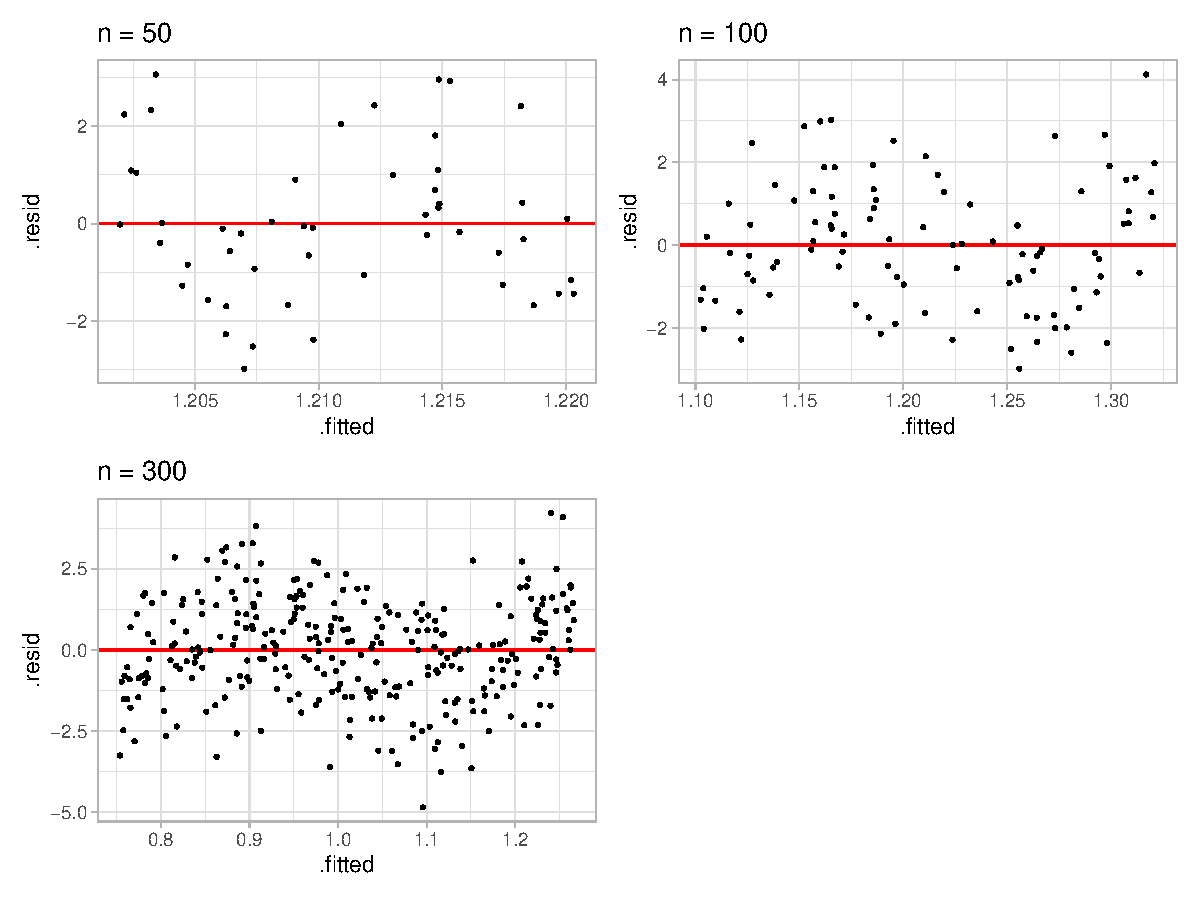
\includegraphics[width=1\linewidth]{paper_comparison_files/figure-latex/different-n-1} 

}

\caption{Three different values of $n$ are used in experiment I, II and III to control the strength of the signal.}\label{fig:different-n}
\end{figure}

\begin{figure}

{\centering 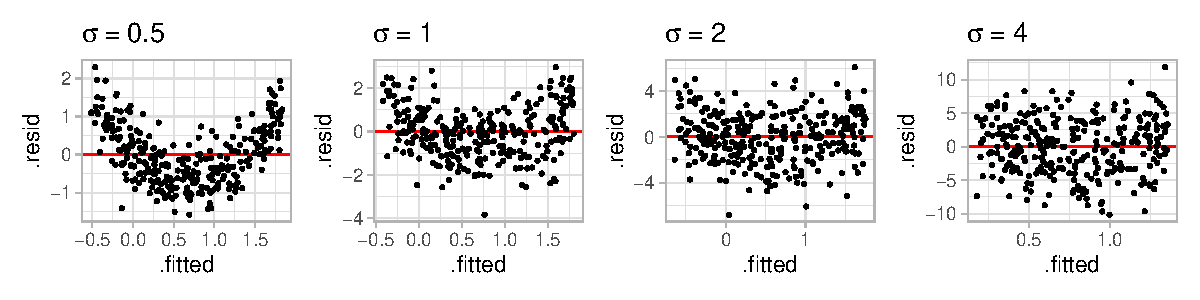
\includegraphics[width=1\linewidth]{paper_comparison_files/figure-latex/different-sigma-1} 

}

\caption{Four different values of $\sigma$ are used in the experiment I to control the strength of the signal.}\label{fig:different-sigma}
\end{figure}

\begin{figure}

{\centering 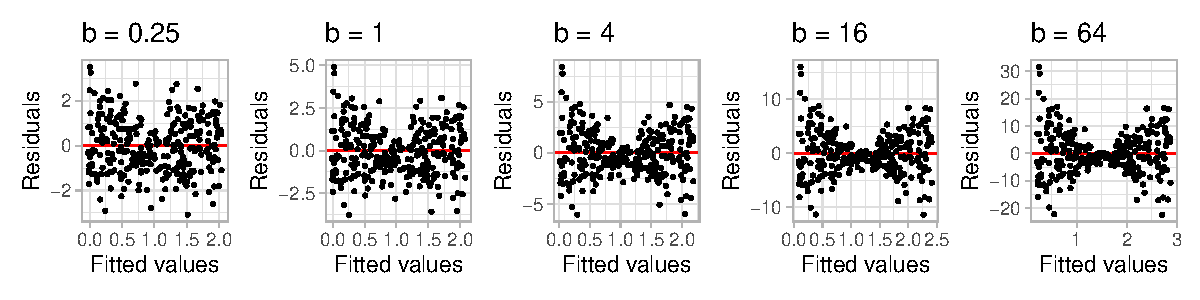
\includegraphics[width=1\linewidth]{paper_comparison_files/figure-latex/different-b-1} 

}

\caption{Five different values of $b$ are used in experiment II to control the strength of the signal.}\label{fig:different-b}
\end{figure}

\hypertarget{subject-allocation}{%
\subsubsection{Subject allocation}\label{subject-allocation}}

Three replications are made for each of the parameter values shown in
Table \ref{tab:parameter-table} resulting in
\((4 \times 4 \times 4 \times 3 + 4 \times 3 \times 5 \times 3) \times 3 = 1116\)
different lineups. In addition, each lineup is designed to be evaluated
by five different subjects. After attempting some pilot studies
internally in our research group, we decide to present a block of 20
lineups to every subject. And to ensure the quality of the survey data,
two lineups with obvious visual patterns are included as attention
checks. Thus, \(576 \times 5/(20-2) = 160\) and
\(540 \times 5 /(20-2) = 150\) subjects were recruited to satisfy the
design of the experiment I and experiment II respectively.

As mentioned in Section {[}the alpha section{]}, \(\alpha\) used in
Equation \ref{eq:eq:pvalue-beta-binomial} needs to be estimated using
Rorschach lineups. Hence, 36 Rorschach lineups with all combinations of
\(n\) and \(X_{raw}\) and three replications are designed to be included
in experiment III. All Rorschach lineups are planned to be evaluated by
20 subjects. However, presenting only Rorschach lineups to subjects are
considered to be bad practices as subjects will lose interest quickly.
We planned to also collect 6 more evaluations on the 279 lineups with
uniform distribution, resulted in
\((36 \times 20 + (4 \times 4 \times 3 + 3 \times 5 \times 3) \times 3)/(20-2) = 133\)
subjects recruited for experiment III.

\hypertarget{collecting-results}{%
\subsubsection{Collecting results}\label{collecting-results}}

Subjects for all three experiments were recruited from an crowdsourcing
platform called Prolific {[}ref here{]}. Prescreening procedure was
applied during the recruitment, subjects were required to be fluent in
English, with \(98\%\) minimum approval rate in other studies and 10
minimum submissions. During the experiment, every subject was presented
with a block of 20 lineups. For each lineup, the actual data plot was
drawn as a standard residual plot of the null model with raw residuals
on the y-axis and fitted values on the x-axis. An additional horizontal
red line was added at \(y = 0\) as a helping line. The 19 null datasets
were generated by the residual rotation technique, and plotted in the
same way. The lineup consisted of 20 residual plots with one randomly
placed actual data plot. And for every lineup, the subject was asked to
select one or more plots that are most different from others, provide a
reason for their selections, and evaluate how different they think the
selected plots were from others. If there was no noticeable difference
between plots in a lineup, subjects were permitted to select zero plots
without providing the reason. No subject was shown the same lineup
twice. Information about preferred pronoun, age group, education, and
previous experience in visual experiment were also collected. A
subject's submission was only accepted if the actual data plot was
identified for at least one attention check. Data of rejected
submissions were discarded automatically to maintain the overall data
quality.

\hypertarget{results}{%
\section{Results}\label{results}}

\hypertarget{data-overview}{%
\subsection{Data overview}\label{data-overview}}

There were 2880, 2880 and 2214 lineups evaluation made by 160, 160 and
123 subjects recruited for experiment I, II and III respectively. In the
total of 7974 lineup evaluations, 3744 used lineups produced by the
non-linearity model, 3510 used lineups produced by the
heteroskedasticity model, and 720 used lineups consists of only null
plots.

Besides, there were 886 attention checks not included in the following
analysis. The collated dataset is provided in \texttt{vi\_survey} of the
\texttt{visage} \texttt{R} package.

\hypertarget{p-value-comparison}{%
\subsection{P-value comparison}\label{p-value-comparison}}

Visual inference and conventional hypothesis testing are two distinct
statistical procedures. As displayed in Figure
\ref{fig:p-value-comparison}, the visual test gives higher p-values than
the conventional test for both polynomial and heteroskedasticity models
in most of the time, suggesting that humans have lower confidence and
much higher tolerance of the residual departures than the conventional
test.

In particular, given 95\% confidence level, both tests will reject
\(H_0\) in only around 58\% of the cases. And in 41\% of the cases, the
visual test does not reject \(H_0\) but the conventional test does.
Since fail to reject \(H_0\) in a visual test means that there is no
obvious visual discoveries found in the residual plot, analysts and the
general public as the consumers of the output may not fully believe in
the rejection of \(H_0\) even though the alternative hypothesis is true.
Even if the rejection is accepted, the model violation may not be
considered as impactful due to the fact that the departures are not
clearly visible.

This makes it sounds like people are arrogantly ignoring the accuracy of
conventional tests and trust too much to their visual perception, but it
is not. In fact, the sensitivity of the conventional test could
sometimes distract and discourage analysts from finding a simple but
good linear approximation to the data. The rejection of \(H_0\) because
of acceptable and negligible residual departure is not practically
meaningful and useful. This also partly explains why abundance of
literature suggesting the use of data plot in regression diagnostics.

\begin{figure}

{\centering 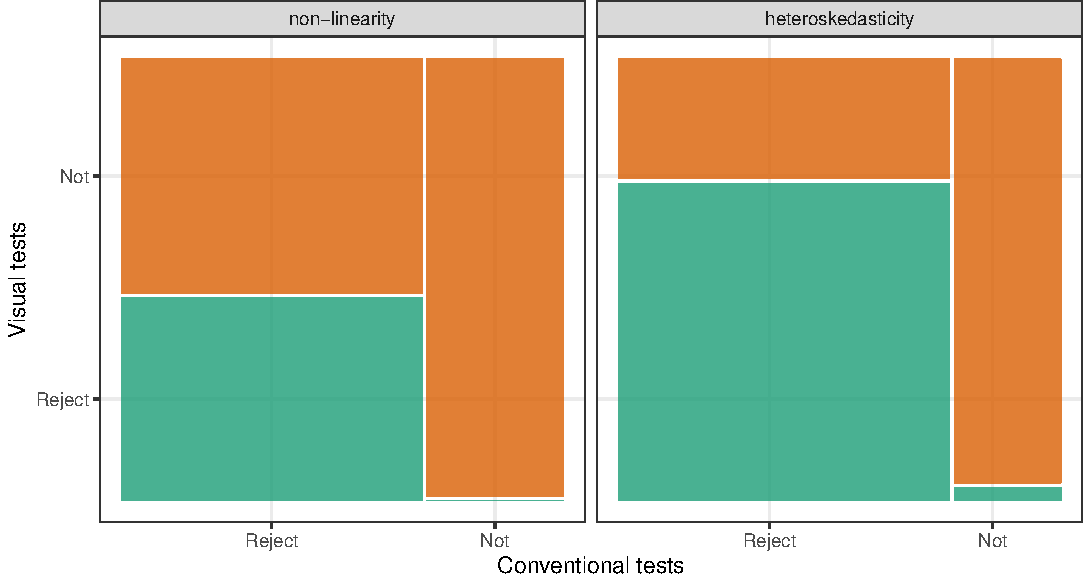
\includegraphics[width=1\linewidth]{paper_comparison_files/figure-latex/p-value-comparison-1} 

}

\caption{Visual test p-value compared to conventional test p-value for lineups produced by heteroskedasticity and non-linearity model. The scatter plot is drawn on a square root scale. Every dot on the plot corresponds to a lineup. Most of the dots are fallen on the left of the y = x line indicating visual test p-value is almost always higher than conventional test p-value. The blue curve is a smoothing of the dots showing a positive trend. }\label{fig:p-value-comparison}
\end{figure}

\hypertarget{power-comparison}{%
\subsection{Power comparison}\label{power-comparison}}

Figure \ref{fig:polypower} show the estimated power of visual test on
lineups produced by the non-linearity model with the \(X_{raw}\)
following a uniform distribution, against the natural logarithm of the
effect \(log_e(E)\) with comparison to the power of an exact test -
F-test, and two other residual-based conventional tests commonly used in
regression diagnostics but for testing heteroskedasticity and
non-normality respectively. At the bottom of the figure
\ref{fig:polypower}, there are a sequence of example residuals plots
with increasing levels of \(log_e(E)\). Readers can evaluate them from
left to right and determine at which level the departure from a good
residual plot becomes detectable.

Figure \ref{fig:heterpower} is similar to Figure \ref{fig:polypower},
but shows corresponding information on lineups produced by the
heteroskedasticity model. In this scenario, the visual test is compared
to an approximate test - Breusch-Pagan test, and two other inappropriate
tests - F-test and Shapiro-Wilk test.

For the non-linearity model, the power of all four tests increases as
the effect gets larger. The power curve of F-test climbs aggressively
from 25\% to around 90\% as \(log_e(E)\) increases from 0 to 2, while
power of other tests respond inactively to the change of effect and
remain lower than 25\% throughout the period, showing that F-test is way
more sensitive to the type of model defects that being considered.
Meanwhile, no noticeable visual features can be spotted from the example
residuals plots.

In terms of the heteroskedasticity model, the power of Breusch-Pagan
test is also almost always greater than the power of visual test. For
\(0 \leq log_e(E) \leq 2\), where the visual feature is nearly
unobservable from the example residual plots and the power curve of the
visual test remains at a low level, the Breusch-Pagan test still have a
decent amount of chance of rejecting \(H_0\).

The power of visual test arises steadily as \(log_e(E)\) increases from
2 to 5 in both non-linearity model and heteroskedasticity model,
suggesting that the effect starts to make significant impact on the
degree of the presence of the designed visual features. This can also be
observed from the example residuals plots that when \(log_e(E) = 2.5\),
a weak ``S-shape'' and a weak ``triangle'' shape are presented in Figure
\ref{fig:polypower} and Figure \ref{fig:heterpower} respectively. And as
\(log_e(E)\) increases, the visual pattern becomes much clearer, and the
power reaches almost 100\% at \(log_e(E) \approx 6\).

The power of all inappropriate tests except for F-test shows improvement
as the effect increases but at a lower rate than the visual test in both
scenarios. This coincides the point made by \citet{cook1982residuals}
that residual-based tests for a specific type of model defect may be
sensitive to other types of model defects. The power curve of F-test
remains at around 5\% in Figure \ref{fig:heterpower} since there is no
non-linear term leave out in the heteroskedasticity model and \(H_0\) of
the F-test will be always satisfied.

Overall, the power analysis suggests that conventional tests do not
match how humans perceive residual plots and thus determine model
violations in these two scenarios. Non-severe model violations with
human acceptable residual departures could often alarm by the
conventional tests. This could limit the popularity of conventional
tests in residual diagnostics among analysts.

\begin{figure}

{\centering 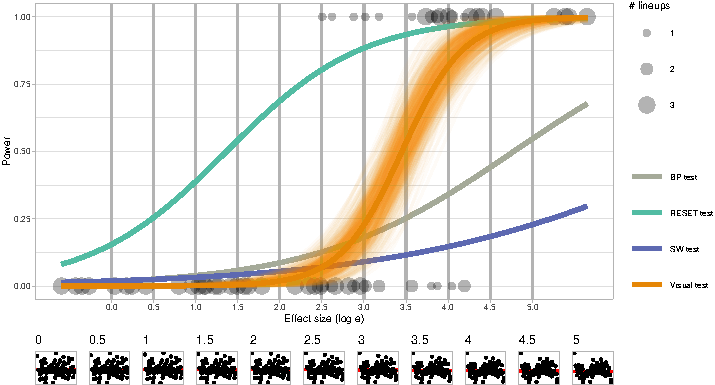
\includegraphics[width=1\linewidth]{paper_comparison_files/figure-latex/polypower-1} 

}

\caption{Comparison of power between different tests for nonlinear patterns. Main plot shows the power curves, with dots indicating human evaluations of lineups. Small row of plots shows typical residual plots corresponding to specific effect sizes, marked by dashed lines in main plot. Where would you draw the line of too much nonlinearity in the residuals? For the F test this is around log effect size 0.5, but for the visual test it is around 3.}\label{fig:polypower}
\end{figure}

\begin{figure}

{\centering 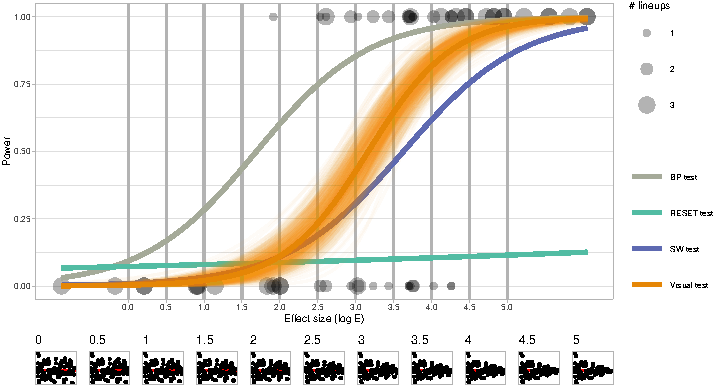
\includegraphics[width=1\linewidth]{paper_comparison_files/figure-latex/heterpower-1} 

}

\caption{...}\label{fig:heterpower}
\end{figure}

\hypertarget{lineup-selection}{%
\subsection{Lineup selection}\label{lineup-selection}}

\begin{figure}

{\centering 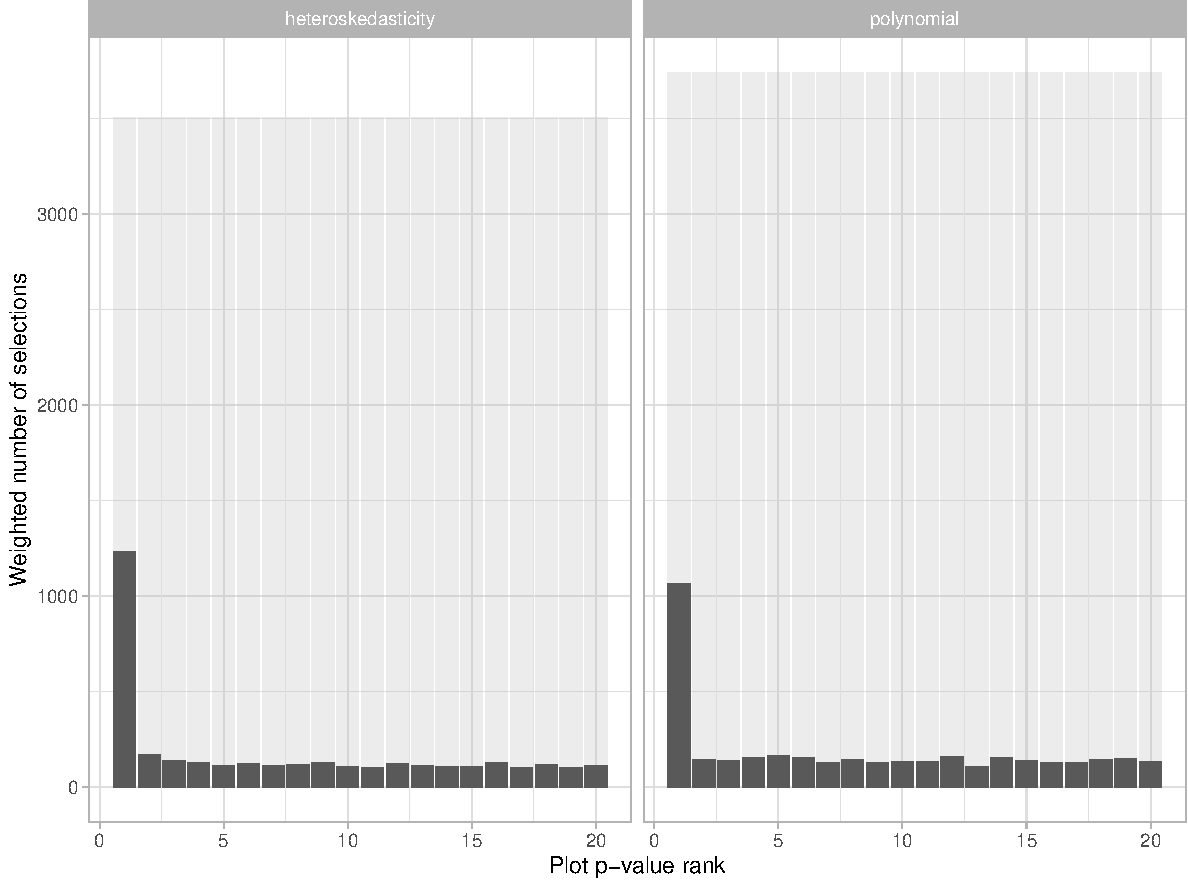
\includegraphics[width=1\linewidth]{paper_comparison_files/figure-latex/plotsel-1} 

}

\caption{A large amount of subjects select the residuals plot with the lowest p-value. But greater than 50 percent of subjects evenly select other plots.}\label{fig:plotsel}
\end{figure}

\begin{figure}

{\centering 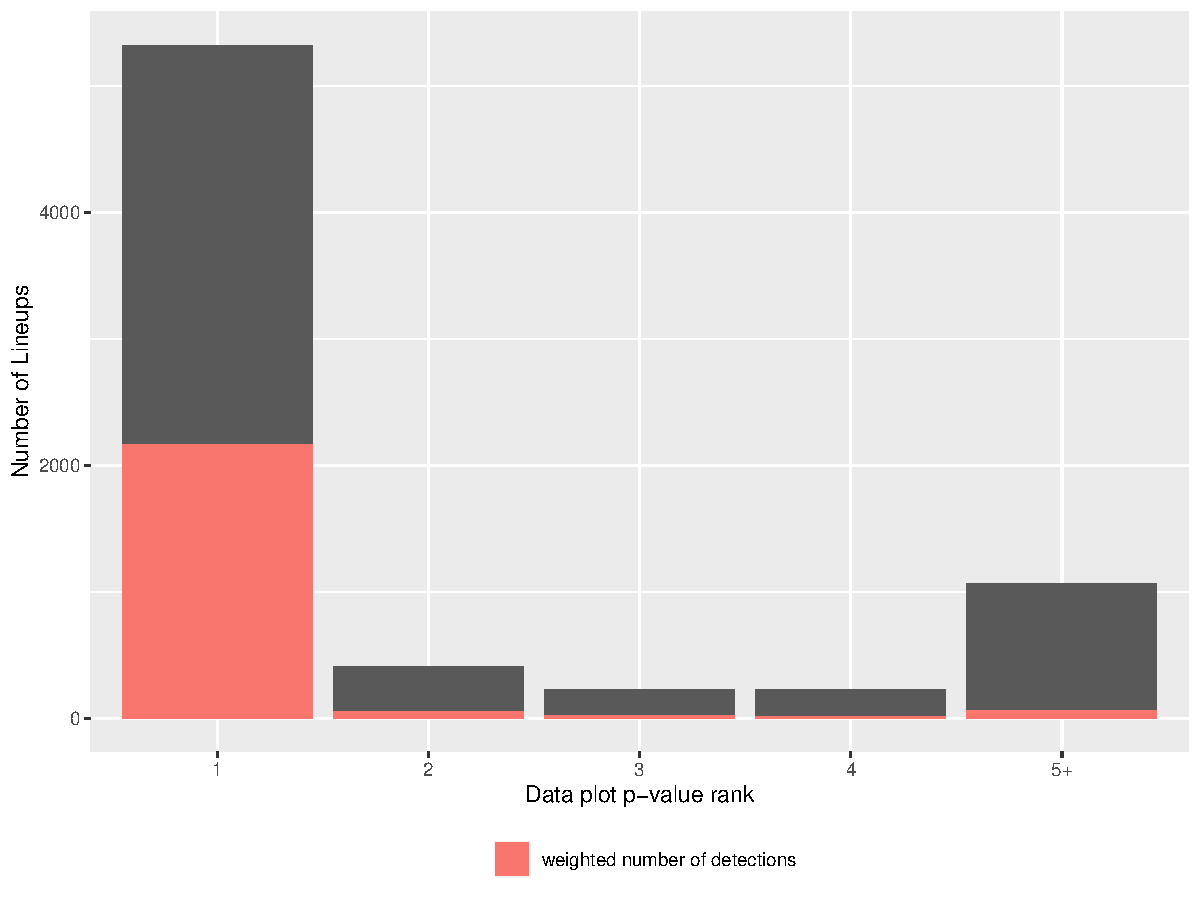
\includegraphics[width=1\linewidth]{paper_comparison_files/figure-latex/dataplotsel-1} 

}

\caption{...}\label{fig:dataplotsel}
\end{figure}

\begin{figure}

{\centering 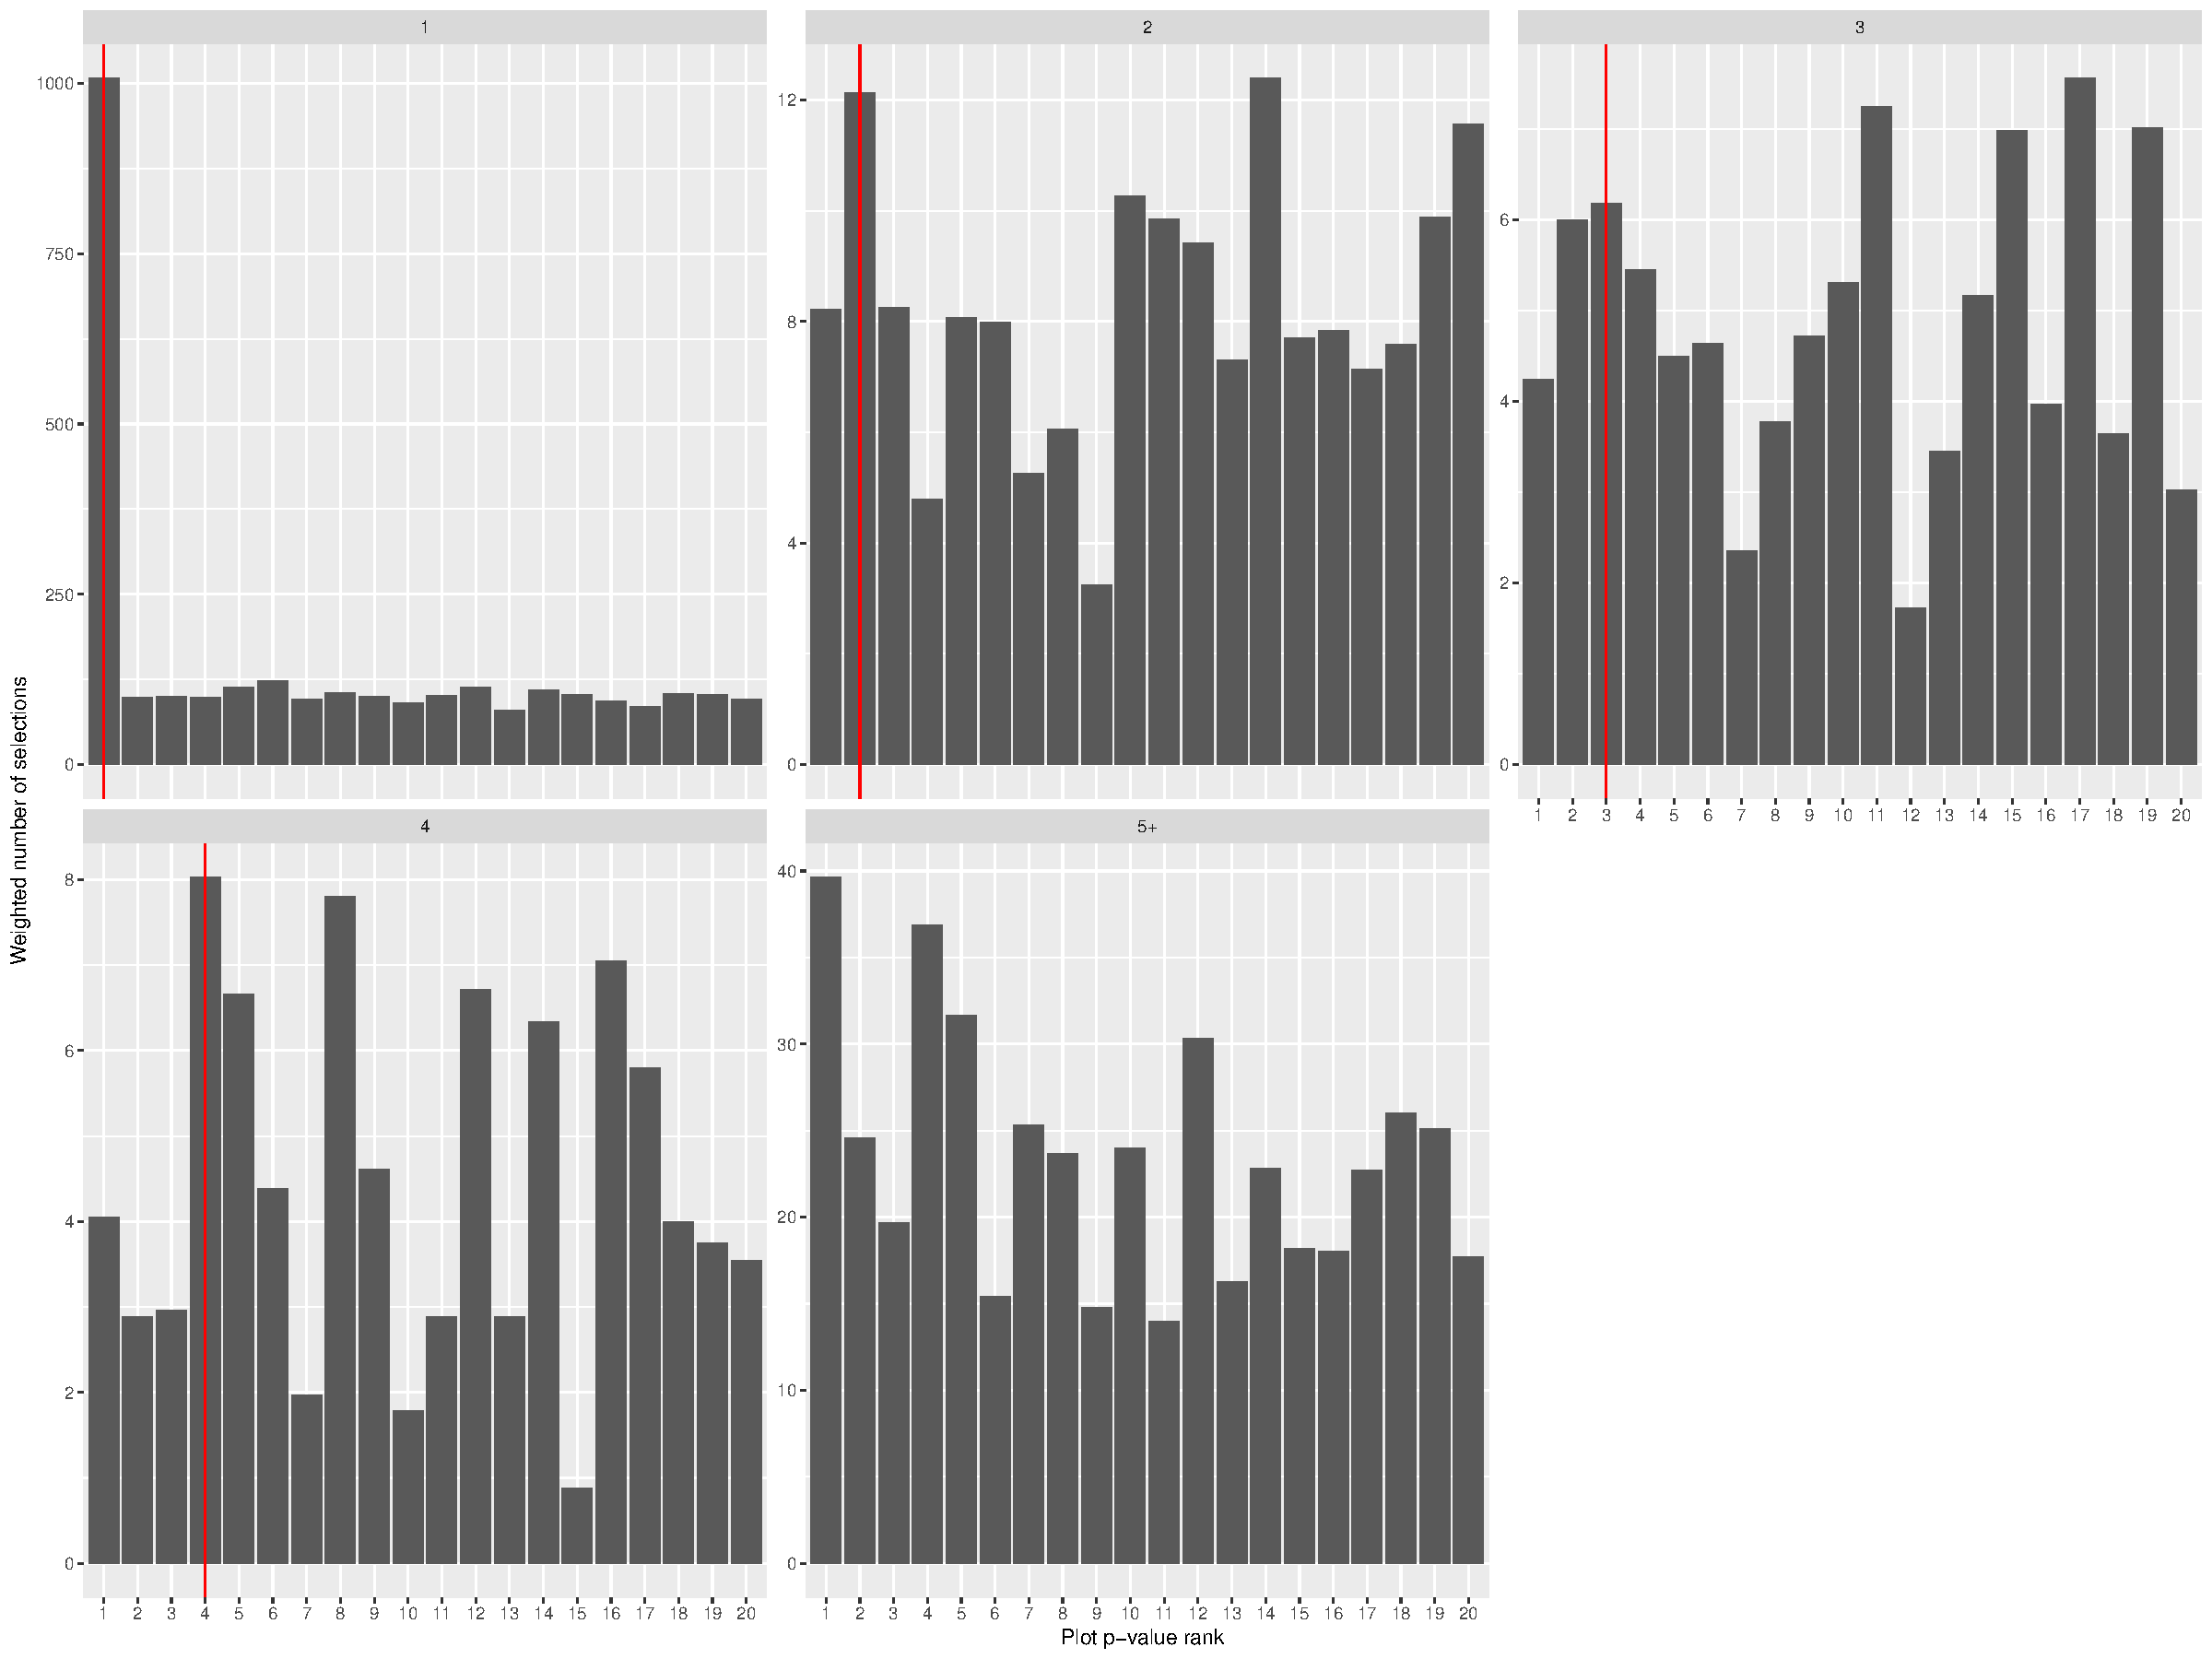
\includegraphics[width=1\linewidth]{paper_comparison_files/figure-latex/dadtaplotselfacet-1} 

}

\caption{...}\label{fig:dadtaplotselfacet}
\end{figure}

\bibliographystyle{tfcad}
\bibliography{paper.bib}





\end{document}
